\chapter{Implementation} % Chapter 2
%

%\nocite{*}

\section{Introduction} % a.
This chapter looks at the high level and low level views of the system. The high level view provides an outline of the processes followed during the implementation of the system, while the low level view provides a more detailed description. 

\begin{figure}[H]
  \centering
  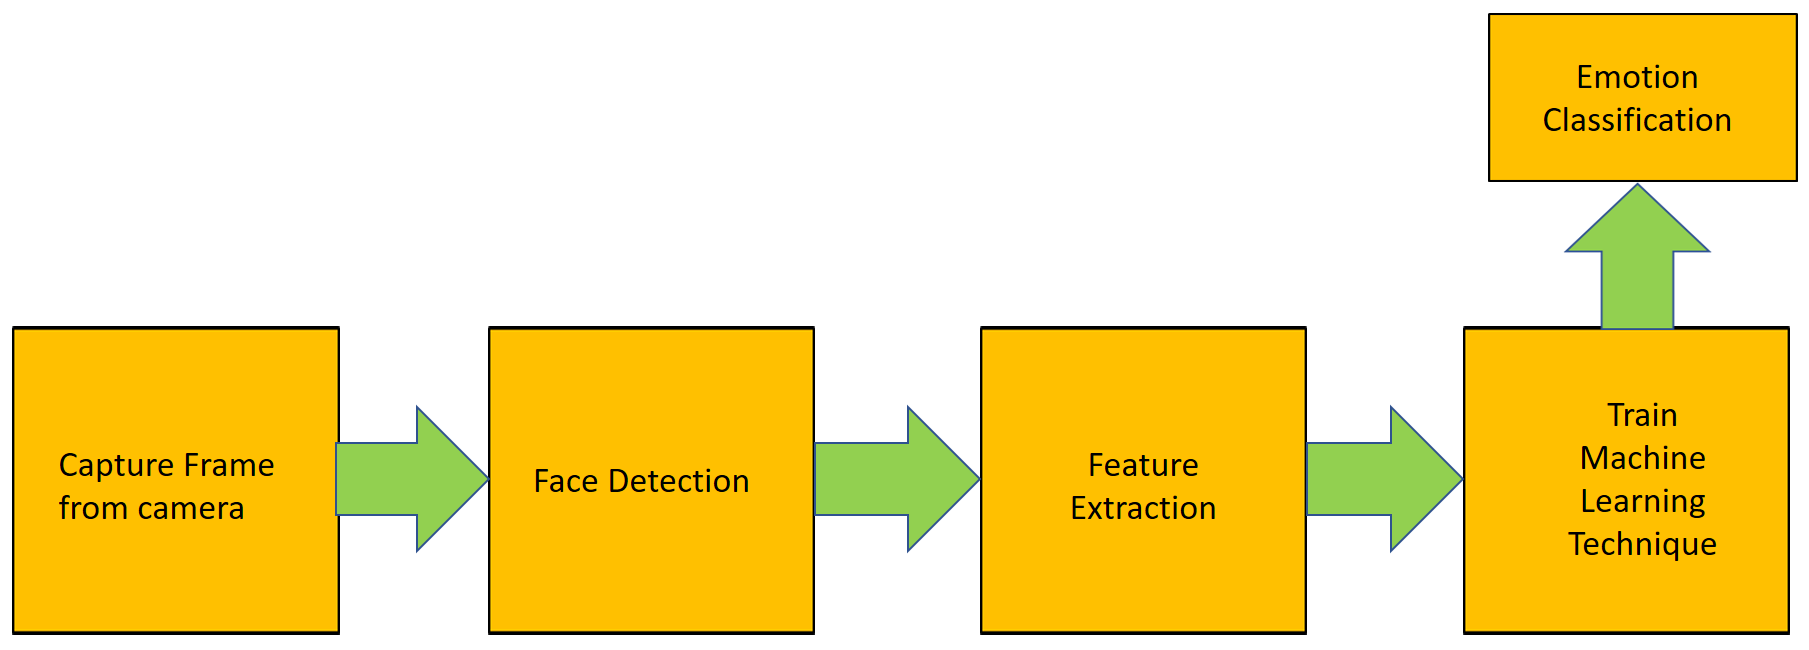
\includegraphics[scale=0.2]{pres1}
  \caption{High level view of System}
\end{figure} 
Looking at \textit{Figure 4.1}, the High level view is explained by:

\begin{itemize}
  \item Capture Frame - The web camera records a constant stream of video input. The video input consists of a sequence of multiple image frames. The system captures each frame for processing as it is displayed on the video feed.

  \item Face Detection - Now that we have captured a single frame, we need to check if there is a face present in the frame. This is done using a face detection algorithm. If a face is present in the frame, the location of the face is extracted.

  \item Feature Extraction - Every emotion displayed facially has it's own set of unique identifying features. By applying feature extraction we are able to represent these features in a way that a computer can understand and process. The feature extraction method is applied to the region of the image that contains the face.

  \item Train Machine Learning Technique - Machine learning is a method used by computers to learn how to identify patterns in a given set of features. This process is called training. When we train the system, our features are labeled (Happy, Sad, Angry etc.). Labeling the features helps guide the computer in the learning process.

  \item Emotion Classification - When the training is complete, classification helps to test the accuracy of the trained model. At this point the model should be able to identify emotions given unlabeled features.
\end{itemize}
A visual representation of how the high level view relates to the image processing techniques discussed in Chapter 3 is presented in\textit{Figure 4.2}. 
\begin{figure}[H]
  \centering
  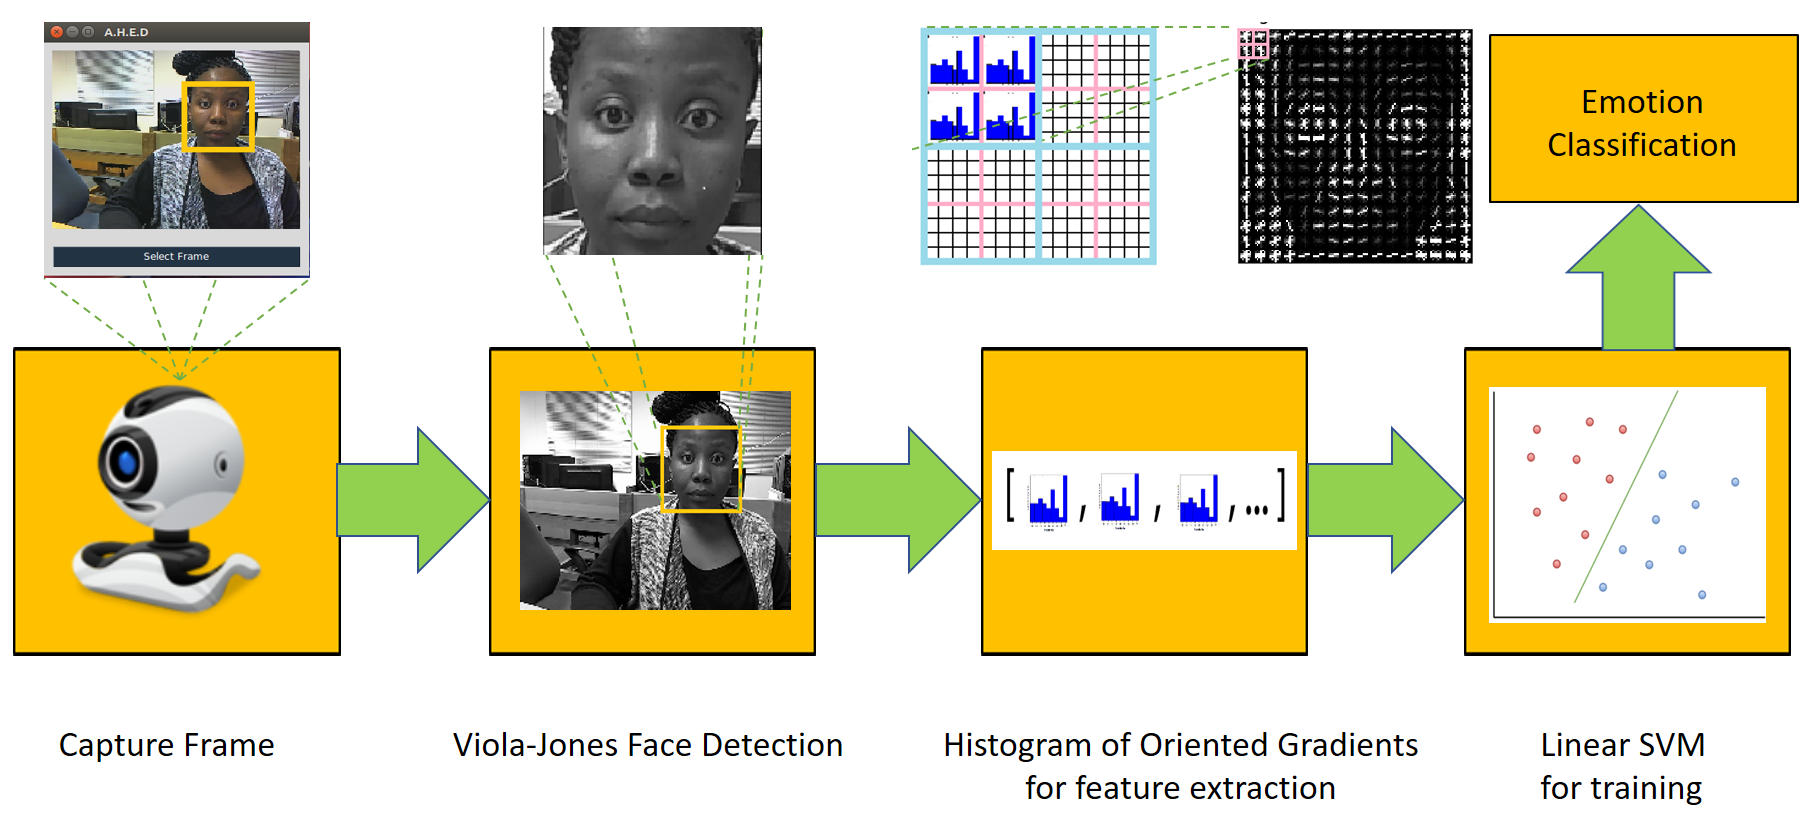
\includegraphics[scale=0.2]{pres2}
  \caption{Low level view of System}
\end{figure} 
